\documentclass[a4paper,twocolumn]{article}
\usepackage[margin=2.75cm]{geometry}
\usepackage[utf8]{inputenc}
\usepackage[portuguese]{babel}
\usepackage{amsmath}
\usepackage{cite}
\usepackage{hyperref}
\usepackage[final]{pdfpages}

\setlength{\columnsep}{0.75cm}

\title{Segundo Mini Projeto de Língua Natural \\\medskip \small Grupo 21}
\author{Duarte Teles \\ 83450 \and Ricardo Brancas \\ 83557 \and Daniel Oliveira \\ 87848}

\begin{document}

\maketitle

\section{Introdução}

O objetivo deste projeto é desenvolver uma métrica de similaridade que permita classificar, em relação ao tipo, questões dadas sobre cinema.
Por exemplo: a classificação da pergunta \textit{``What are the most relevant actors in Bad Boys?''} é \texttt{actor\_name}.

Para o desenvolvimento da nossa solução, utilizaremos um \textit{corpus} pré-etiquetado (\texttt{QuestoesConhecidas.txt}) para treinar o nosso classificador; um conjunto de \textit{embeddings} pré-treinados (ver secção~\ref{embeddings}) e ainda um \textit{corpus} de desenvolvimento (\texttt{NovasQuestoes.txt}).

\section{Arquitetura do Modelo}

\subsection{Pré-Processamento}

O nosso corpus de treino consiste num conjunto de pares $ \langle \text{classificação}, \text{pergunta} \rangle $.
De modo a minimizar o ruído provocado por partes pouco relevantes da frase, realizamos vários passos de pré-processamento, tanto para o \textit{corpus} de treino, como para o novo conjunto de questões a classificar:
\medskip

Por cada um dos ficheiros da pasta \texttt{recursos} (com a exceção do ficheiro \texttt{list\_keywords.txt}), substituimos qualquer ocorrência das palavras contidas no mesmo por uma única palavra genérica.
Por exemplo, todos os títulos de filmes conhecidos são substituídos pela palavra \texttt{movie}. Isto impede o classificador de fazer \textit{overfitting} aos nomes próprios contidos no \textit{corpus} de treino.
Excluímos o ficheiro \texttt{list\_keywords.txt} porque continha várias palavras que são importantes para a nossa tarefa, como por exemplo a palavra \texttt{actors}.
\medskip
    
De seguida segmentamos a frase obtida, removendo toda a pontuação e números existentes, obtendo uma lista de \textit{tokens} que é depois filtrada com recurso às \textit{stop words} do \texttt{NLTK}\label{nltkusage}.
Estas \textit{stop words} consistem num conjunto de palavras comuns que para a nossa tarefa não possuem significado relevante. Alguns exemplos: \texttt{me}, \texttt{you}, \texttt{that'll}, \texttt{now}.
\medskip

Por fim eliminamos todas as palavras para as quais não possuímos um \textit{embedding}, visto que não seria possível relacioná-las de qualquer modo.

\subsection{Obtenção dos \textit{Embeddings}} \label{embeddings}

As palavras do vocabulário de um sistema de Língua Natural podem ser representadas de várias formas e, dependendo dessa representação, pode ou não ser possível estabelecer-se uma relação semântica entre diferentes palavras.

Uma possível representação para os nossos símbolos (palavras) que permite estabelecer relações de semântica é a utilização de \textit{Vector Space Models} \cite{DBLP:conf/emnlp/ErkP08}. A representação de palavras num espaço vetorial contínuo permite mapear palavras com significado semântico semelhante em zonas próximas do espaço. Esta assunção é baseada na \textit{Distributional Hypothesis} \cite{DBLP:conf/cogsci/DyeJYR17} que afirma que palavras que ocorram em contextos semelhantes têm semântica semelhante.

As abordagens que utilizam este principio são \textit{count based methods} e \textit{predictive methods}. O primeiro calcula a co-ocorrência de palavras com os seus vizinhos e mapeia estas contagens num vetor denso para cada palavra. Os modelos preditivos tentam prever diretamente a ocorrência de uma palavra dado os vizinhos de acordo com os vários contextos em que cada palavra ocorre.
\medskip

Assim, de modo a extrair semântica de cada frase e relacionar essa semântica com os tópicos correspondentes, utilizamos um modelo de \textit{embeddings}\label{modelusage} \cite{google_w2v} obtidos através de \texttt{WordToVec} \cite{DBLP:journals/corr/abs-1301-3781}.

Este modelo baseia-se no método preditivo, em particular na arquitetura de modelo \textit{Continuous Bag of Words} \cite{DBLP:journals/corr/abs-1301-3781}, no qual a ordem das palavras não importa e onde existe uma janela sobre a frase através da qual as palavras vizinhas são utilizadas para tentar estimar a melhor codificação de forma a prever cada palavra no corpus de treino, utilizando os múltiplos contextos em que a mesma ocorre.

\subsection{Semântica da Frase}
No modelo de \textit{embeddings} que estamos a utilizar, o conteúdo semântico está ao nível da palavra. Para extrair semântica da frase, com o modelo  aqui apresentado, é necessário combinar os \textit{embeddings} das palavras da frase de algum modo.
Uma das formas mais simples de o fazer consiste apenas em somar os \textit{embeddings} das diferentes palavras e depois normalizar, o que dará origem a um único vetor para cada frase.
\medskip

Esta abordagem tem a vantagem de ser mais simples que outras apresentadas no trabalho futuro ao nível da complexidade computacional, mas traz também alguns  problemas. Em particular, qualquer palavra ou carácter na frase, desde que tenha um \textit{embedding} pré treinado, irá ter um peso equivalente a qualquer outra palavra. Isto é mitigado através do pré-processamento realizado, mas seria útil ter a possibilidade de pesar as palavras de uma forma mais generalizada.

\subsection{Medida de Similaridade}
Como medida de similaridade entre frases (representadas como vetores) foi utilizado o cosseno. Este funciona como uma distância euclidiana normalizada, a qual pode ser utilizada no nosso problema pois os valores dos vetores estão normalizados entre $-1$ e $1$.

\section{Análise de Resultados}

\subsection{Ferramentas}
Para obter os resultados apresentados de seguida utilizámos as seguintes ferramentas:
\begin{itemize}
    \item O pacote \texttt{NLTK} e, em particular, o módulo \texttt{stopwords} cuja utilização foi descrita na secção~\ref{nltkusage}.
    
    \item O pacote \texttt{gensim}, utilizado para carregar o modelo e obter o \textit{embedding} das diferentes palavras.
    
    \item O pacote \texttt{scikit-learn}, utilizado para facilitar alguns cálculos matemáticos.
    
    \item O modelo de \textit{embeddings} treinado sobre o \textit{corpus} ``Google News'' usando \textit{Continuos Bag of Words} com vetores de dimensão 300, já referido na secção \ref{modelusage}.
\end{itemize}

\subsection{Resultados}

Na figura~\ref{fig:conf1} apresentamos os resultados obtidos da classificação do \textit{corpus} de teste fornecido; como é possível observar, o nosso classificador atribui categorias corretas para todas as questões, obtendo uma acurácia de $100\%$.
\medskip

\begin{figure}[h]
	\centering
	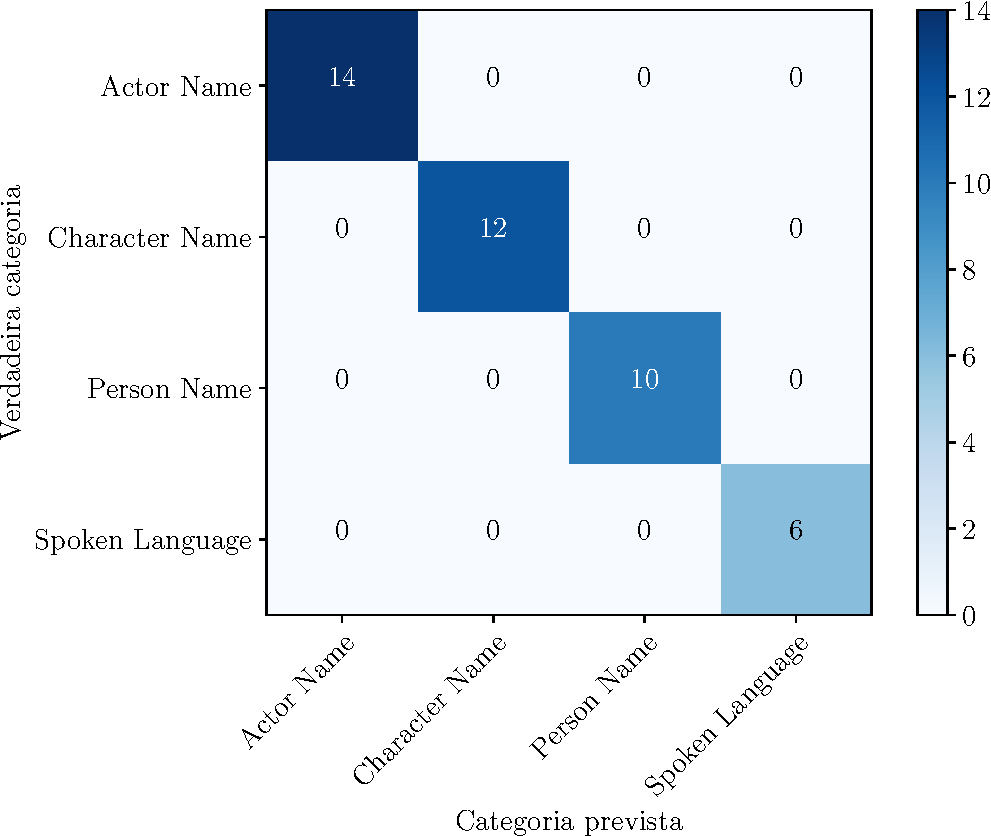
\includegraphics[width=\linewidth]{cm1.pdf}
	\caption{Matriz de confusão para o \textit{corpus} de teste fornecido.}
	\label{fig:conf1}
\end{figure}

Já na figura~\ref{fig:conf2} apresentamos os resultados que obtivemos utilizando um \textit{corpus} de teste estendido por nós. Considerando este conjunto de perguntas mais amplas, incluindo algumas paras as quais temos muito poucos exemplos, a acurácia obtida é $98\%$.

\begin{figure}[h]
	\centering
	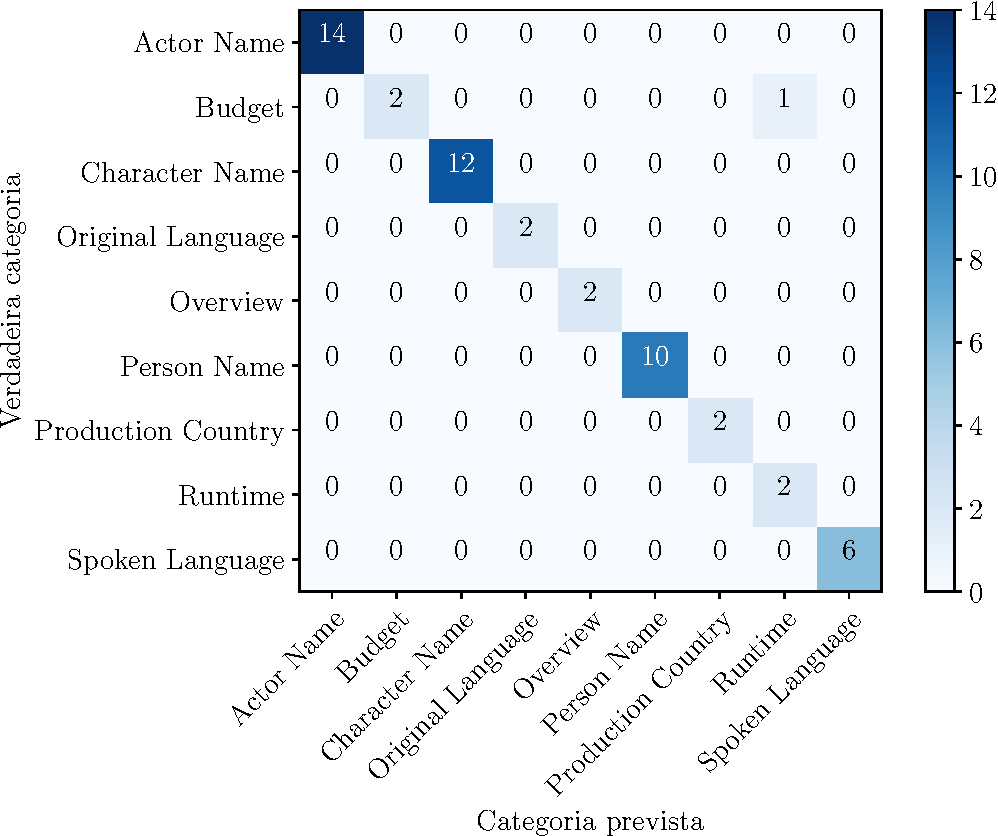
\includegraphics[width=\linewidth]{cm2.pdf}
	\caption{Matriz de confusão para um \textit{corpus} de teste estendido.}
	\label{fig:conf2}
\end{figure}

Experimentámos ainda usar apenas o \textit{subset} do modelo de \textit{embeddings} incluído com o \texttt{NLTK}, obtendo uma acurácia de $97\%$ no \textit{corpus} de desenvolvimento original e cerca de $94\%$ no estendido. 

\section{Trabalho Futuro}
De forma a melhorar a prestação do nosso modelo e a resolver o problema que a abordagem \textit{Continuous Bag of Words} nos traz, podemos recorrer a modelos que pesam de forma independente a presença de cada tópico na frase. Um modelo a considerar é o \textit{Latent Dirichlet Allocation} \cite{DBLP:conf/nips/BleiNJ01}, que descreve a distribuição de tópicos por documento. Poderíamos ainda utilizar outras abordagens para resolver o problema tal como \textit{Text Frequency-Inverse Document Frequency}.

\bibliographystyle{plain}
\bibliography{references}

\end{document}
